\documentclass[12pt,oneside, letterpaper]{book}
\usepackage[utf8]{inputenc}
\usepackage{indentfirst}
\usepackage{setspace}
\usepackage{titlesec}
\usepackage{ragged2e}
\usepackage{setspace}
\usepackage{tabu}
\usepackage{geometry}

% Set margins
\geometry
{a4paper,
	top=2.0in,
	bottom=1.0in,
	left=1.5in,
	right=1.0in,
	headsep=0.0in,
	footskip=0.5in
}

% For inserting images
\usepackage{graphicx}
\graphicspath{ {./Images/} }

% For the references
\usepackage[sorting=none]{biblatex}
%\addbibresource{References.bib}

% Setting page numbers
\pagestyle{plain}
\pagenumbering{roman}
\justifying

% For making the list of abbreviations
\usepackage{nomencl}
\makenomenclature
\renewcommand{\nomname}{List of Abbreviations}

\begin{document}
% makes the page numbers roman numerals, doesn't count
% these pages in the table of contents


%Begin the title page
\begin{titlepage}
 \begin{center}

THESIS OR DISSERTATION TITLE IS CENTERED AND IN ALL CAPS.\\
THE FIRST LINE OF THE TITLE SHOULD BE TWO INCHES FROM.\\
THE TOP OF THE PAGE. SINGLE-SPACED.

 \vspace{6.5cm} 
 
BY

\vspace{0.7cm}

AUTHOR NAME IN ALL CAPITAL LETTERS 

\vspace{0.7cm}

B\textit{X}, College of University, YYYY\\
M\textit{X}, College of University, YYYY
 
\vfill 
\vspace{0.8cm}
 
SPECIFY DISSERTATION OR THESIS

\vspace{0.8cm}

Submitted in partial fulfillment of the requirements for\\
the degree of Name of Degree in Major\\
in the Graduate School of\\
Binghamton University\\
State University of New York\\
YYYY
  
   \end{center}
\end{titlepage}

%Begin the copyright page
\newpage

\thispagestyle{empty}

\vbox to 8.0truein{}

\centerline{\copyright\ Copyright by Full Legal Name of Author YYYY}

\

\centerline{All Rights Reserved}

%Begin the committee member page
\newpage
\addtocounter{page}{1}

{\baselineskip = 10pt

\vbox to 5.5truein{}

\centerline{Accepted in partial fulfillment of the requirements for}
\centerline{the degree of Name of Degree in Major}
\centerline{in the Graduate School of}
\centerline{Binghamton University}
\centerline{State University of New York}
\centerline{YYYY}

\

\centerline{Month DD, YYYY}

\

\centerline{First Name Last Name, Chair}
\centerline{Department of XXXXXX, University Name}
\

\centerline{First Name Last Name, Faculty Advisor}
\centerline{Department of XXXXXX, University Name}
\

\centerline{First Name Last Name, Member}
\centerline{Department of XXXXXX, University Name}
\

\centerline{First Name Last Name, Outside Examiner}
\centerline{Department of XXXXXX, University Name}
}


\newpage
\newgeometry
{a4paper,
	top=1.0in,
	bottom=1.0in,
	left=1.5in,
	right=1.0in,
	headsep=0.0in,
	footskip=0.5in
}
\newcommand{\chapfnt}{\fontsize{18}{18}}
\newcommand{\secfnt}{\fontsize{14}{14}}
\newcommand{\ssecfnt}{\fontsize{12}{12}}
\setstretch{2.0}
 
\titleformat{\chapter}[hang]
{\normalfont\chapfnt\bfseries\centering}{\thechapter\ }{1em}{}
\titlespacing*{\chapter}{0pt}{1in}{12pt}

\titleformat{\section}
{\normalfont\secfnt\bfseries}{\thesection}{1em}{}
 
\titleformat{\subsection}
{\normalfont\ssecfnt\bfseries}{\thesubsection}{1em}{}

\chapter*{Abstract}
\par The abstract is mandatory.
\par The maximum acceptable length for an abstract to be published in Dissertation Abstracts International (DAI) is 350 words. The maximum acceptable length for an abstract to be published in Master’s Thesis Directories (MTD) is 150 words. However, an abstract within the dissertation or thesis need not be limited. The student may prepare a lengthy abstract for inclusion in the thesis or dissertation and a more concise summary for publication in DAI/MTD. 
\par The abstract is expected to give a succinct account of the student's work so that a reader can quickly learn the essential contents and results. A typical abstract includes a statement of the problem, an account of procedure or methods followed, and an account of main results and conclusions.
\par Abstracts must be prepared carefully, since they are published in DAI/MTD without editing or revision.

\newpage

\vbox to 4.25truein{}
\centerline{The dedication is optional. Type your dedication here, centered on the page.}

\newpage
\begin{doublespace}
\chapter*{Acknowledgements}
\par The Acknowledgements section is optional. Here, type your acknowledgements. Double-space. If your style guide of choice (e.g., MLA, APA, Chicago, etc.) gives specific formatting guidelines, follow them.
\end{doublespace}

\newpage
\begin{doublespace}
\chapter*{Preface}
\par The preface is optional. If necessary, the following information should be included:
\par For previously published works, cite each published piece fully and indicate whether your studies or articles are being republished in their entirety and in the original wording, or whether they have been revised for the dissertation. Indicate that your studies or articles are being included because they were part of the programmatic line of research that comprised the dissertation and that including them provides a coherent and appropriately sequenced investigation. Describe your (the dissertation author) role in the published work. Certify that permission to republish these works in the dissertation has been obtained from the publisher or owner. 
\par For images, identify the ones for which permission has been received by figure number and with reference to the copyright holder (whether an individual or institution) and certify that permission has been obtained. You may wish to add that all other images are in the public domain or being used under a public license or fair use. 
\end{doublespace}
\newpage

\setstretch{1.0}
\tableofcontents
\listoftables
\addcontentsline{toc}{chapter}{List of Tables}

\listoffigures
\addcontentsline{toc}{chapter}{List of Figures}

\addcontentsline{toc}{chapter}{List of Abbreviations}
\chapter*{List of Abbreviations}
Include any listing of abbreviations on this page.
%\printnomenclature

\mainmatter
\setstretch{2.0}

\chapter{Introduction}
\par The following text is only included to take up space and provide a visual sense of the layout of your paper.   It is written in Latin for no reason other than to encourage you to bypass it as not being necessary information for you to spend your time reading.  
\par Sed ut perspiciatis unde omnis iste natus error sit voluptatem accusantium doloremque laudantium, totam rem aperiam, eaque ipsa quae ab illo inventore veritatis et quasi architecto beatae vitae dicta sunt explicabo. Nemo enim ipsam voluptatem quia voluptas sit aspernatur aut odit aut fugit, sed quia consequuntur magni dolores eos qui ratione voluptatem sequi nesciunt. Neque porro quisquam est, qui dolorem ipsum quia dolor sit amet, consectetur, adipisci velit, sed quia non numquam eius modi tempora incidunt ut labore et dolore magnam aliquam quaerat voluptatem. Ut enim ad minima veniam, quis nostrum exercitationem ullam corporis suscipit laboriosam, nisi ut aliquid ex ea commodi consequatur? Quis autem vel eum iure reprehenderit qui in ea voluptate velit esse quam nihil molestiae consequatur, vel illum qui dolorem eum fugiat quo voluptas nulla pariatur?

\chapter{Background and Related Work}
\par Each chapter should begin at the top of a new page, with a two-inch top margin.\footnote{This is your first footnote, if your chosen style manual calls for footnotes rather than endnotes. \\} 
\par Lorem ipsum dolor sit amet, consectetur adipisicing elit, sed do eiusmod tempor incididunt ut labore et dolore magna aliqua. Ut enim ad minim veniam, quis nostrud exercitation ullamco laboris nisi ut aliquip ex ea commodo consequat. Duis aute irure dolor in reprehenderit in voluptate velit esse cillum dolore eu fugiat nulla pariatur. Excepteur sint occaecat cupidatat non proident, sunt in culpa qui officia deserunt mollit anim id est laborum.\footnote{This is your second footnote. There should be a space, as shown, between each note (whether footnote or endnote).}

\section{Media, Politics, and Perception of Crime}
\par TODO: papers about historical media and crime, modern issues, social media effects

\section{Geography}
\par TODO: explanation of geographical terms (urban areas, MSAs, etc)

\section{Reddit as Social Media}
\par TODO: what reddit is and its role in misinformation

\begin{figure}[ht]
    \centering
    \begin{minipage}[t]{0.8\textwidth}
    \textit{Follow this list to ensure your pages are in the correct order. \\}
	\begin{enumerate}
	    \item Title page (mandatory)
	    \item Copyright notice (mandatory)
	    \item Committee page (mandatory)
	    \item Abstract (mandatory)
	    \item Dedication (optional)
	    \item Acknowledgments (optional)
	    \item Preface (optional)
	    \item Table of contents (mandatory)
	    \item List of tables (include list if manuscript includes tables)
	    \item List of figures (include list if manuscript includes figures)
	    \item List of plates (include list if manuscript includes plates)
	    \item List of abbreviations (include if needed)
	    \item Body of manuscript (mandatory)
	    \item Appendix(es) (if necessary)
	    \item Notes (include if necessary)
	    \item Bibliography (mandatory)
	\end{enumerate}
	\end{minipage}
    \caption{Sequence of pages for thesis or dissertation.}
	\label{fig:fig-1}
\end{figure}

\chapter{Subreddit-level Analysis}

\section{Data Overview}
\par The subreddit-level analysis requires a variety of different data inputs. These data inputs can be divided into two major subcategories: post and comment data from Reddit itself and data that provide contextual or qualitative information.

\subsection{Reddit Data}
\par The Reddit dataset contains posts from the subreddits of the 384 MSAs of the United States as of March 2020 (REF). Appendix (REF) provides a full list of subreddits used. From this list of subreddits, we scrape and store all posts that users submit. In total, 161,166 posts were gathered between April 5, 2022 and May 31, 2022. (REF - Figure of timeline). The datastore archives posts in two formats. First, posts are written to a system of record to ensure that there is an authoritative data source that can be referenced. Second, pertinent information, such as post title and author, is extracted from the posts data stream and placed in a separate datastore.

(FIG)

\par After storing data, an analysis tool runs to determine if a post is about crime. To do this, a regular expression checks if a post's title or a post's link's URL contains a crime-related keyword. Appendix (REF) lists the keywords used. These keywords were derived from actions that constitute violent crime and their synonyms, as well as generic crime-related words. If the regular expression returns a hit, a flag is raised in the database denoting that the post is about crime. Overall, 6,792 posts are estimated to discuss crime.

\subsection{Contextual Data}
\par A variety of data were utilized to highlight trends in the Reddit posts. One variable that subreddits are compared to is population size of the MSA (REF). These values range from a minimum of 58,639 (Carson City, NV) and a maximum of 20,140,470 (New York-Newark-Jersey City, NY-NJ-PA). MSAs are categorized into four bins based on their size: large, medium, small, and very small. The population cutoffs are 1,000,000, 500,000, and 200,000. The large population contains 56 members, the medium bin contains 54 members, the small bin contains 113 members, and the very small bin contains 161 members. Appendix (REF) contains the populations of all MSAs.

\par Another variable that provides context is the political climate of an MSA. For this, we consider the results of the 2020 election (REF) in terms of the percent of the MSA voting Democrat. These values range from a minimum of 20.2\% (Morristown, TN) to a maximum of 80.9\% (Santa Cruz-Watsonville, CA). The MSAs are categorized into five bins based on their voting results: Very Conservative, Conservative, Moderate, Liberal, and Very Liberal. The percentage cutoffs for the bins are 37.5\%, 47.5\%, 52.5\%, and 62.5\%. The Very Conservative bin contains 112 members, the Conservative bin contains 103 members, the Moderate bin contains 57 members, the Liberal bin contains 73 members, and the Very Liberal bin contains 39 members. Appendix (REF) contains the voting patterns of all MSAs.

\par A third variable that is considered is the documented violent crime rate of each MSA. This data is derived from the FBI's Uniform Crime Reporting statistics (REF) \footnote{Data from the FBI mostly comes from the year that is most recent, 2019. However, not all municipalities report information, so there are slight estimations in the data (REF). Additionally, not all MSAs have documented 2019 data, so 2018 or 2017 data are used instead. The year gathered is documented in Appendix (REF)}. These values range from a minimum of 44.3/100,000 (Bangor, ME) to a maximum of 1,397.2/100,000 (Birmingham-Hoover, AL). Documented crime data is also normalized using min-max normalization so that it can be compared to a similarly normalized crime discussion value from the Reddit data. Appendix (REF) contains the documented crime rate of all MSAs.

\section{Methods}
\par We use one main scraper to gather post data from Reddit. This scraper utilizes multiple different tools to gather disparate pieces of data and place them into two datastores. This scraper prioritizes resilience to ensure that all posts are accounted for. Additionally, the scraper checks for new posts once every hour so that posts can be fetched before a user deletes them or a moderator deletes them. These communities are generally slow moving, with an average of 111 posts an hour between all 384 subreddits.

\par To gather the data, the scraper first sends requests to the Reddit REST API (REF). We use the \texttt{new} endpoint for each subreddit to check the most recent posts. The post last written to the database for each subreddit is cached in a database table so that we can take advantage of the \texttt{after} parameter of the API. This parameter allows us to take posts that have been created since a given post ID. This parameter is especially useful on slower subreddits; without it, we would be performing requests on posts that might be months old. If the cached value does not exist or is not valid, then the most recent hundred posts are gathered. This is the maximum allowable value by the Reddit API.

\par After performing error checking to ensure all of our requests went through, each record is sent to two databases. The first is a CockroachDB database that acts as a system of record. Raw posts are stored here in a simple format: \texttt{id}, \texttt{timestamp}, and \texttt{data}, which is the data retrieved from the Reddit API in JSON format. After writing to CockroachDB, the scraper then writes the JSON data from Reddit to ElasticSearch. ElasticSearch provides quick and efficient text analysis that allows for the extraction of certain keywords in post titles and URLs.

\par The scraper and databases run in Docker containers. Containerization allows the tool, as well as the databases, to run in a clean, isolated environment without worrying about being choked out by other processes. Additionally, the tool-container is scheduled by Kubernetes to allow for a higher degree of availability and resilience. If something unexpected occurs and the tool goes down, it will simply be restarted by Kubernetes. Figure (REF) details the entire data scraping process.

(FIG)

\section{Results}

\subsection{Activity}

\par In total, the Reddit scraper gathered 161,166 posts between 384 subreddits. Posts were collected between April 5th, 2022 to May 31, 2022. Table \ref{table:table-1} details the ten most active subreddits of those monitored. Similarly, Table \ref{table:table-2} lists the ten most active subreddits when normalized by population.

\begin{table}[h!]
    \centering
    \small
    \caption{Most active Metropolitan Areas}
    %\begin{tabu} to 1.0\textwidth {| *{3}{c|} }
    \begin{tabular}{| c | c | c |}
    \hline
    Metropolitan Statistical Area & Number of Posts & Population\\ \hline
    Austin-Round Rock-Georgetown, TX & 4,084 & 2,283,371 \\ \hline
    San Diego-Chula Vista-Carlsbad, CA & 3,265 & 3,298,634 \\ \hline
    Boston-Cambridge-Newton, MA-NH & 3,120 & 4,941,632 \\ \hline
    Denver-Aurora-Lakewood, CO & 2,785 & 2,963,821 \\ \hline
    Chicago-Naperville-Elgin, IL-IN-WI & 2,673 & 9,618,502 \\ \hline
    Sacramento-Roseville-Folsom, CA & 2,668 & 2,397,382 \\ \hline
    Philadelphia-Camden-Wilmington, PA-NJ-DE-MD & 2,541 & 6,245,051 \\ \hline
    Columbus, OH & 2,533 & 2,138,926 \\ \hline
    Portland-Vancouver-Hillsboro, OR-WA & 2,526 & 2,512,859 \\ \hline
    San Francisco-Oakland-Berkeley, CA & 2,476 & 4,749,008 \\ \hline
	\end{tabular}
	\label{table:table-1}
\end{table}

\par The most active MSAs by total number of posts share some common, predictable traits. First, all of the Metropolitan Areas listed have populations above 1,000,000. While expected, some notable MSAs were not included, such as New York-Newark-Jersey City, NJ-NJ-PA and Los Angeles-Long Beach-Anaheim, CA, which have populations of 20,140,470 and 13,200,998, respectfully. One possible explanation for these discrepancies is the fact that there is no uniform, consistent moderation policy among subreddits (REF). For example, some subreddits automatically filter out all posts and manually approve them, or they disallow certain types of posts (REF - nyc n chicago rules).

\begin{table}[h!]
    \centering
    \small
    \caption{Most active Metropolitan Areas per population}
    %\begin{tabu} to 1.0\textwidth {| *{3}{c|} }
    \begin{tabular}{| c | c | c |}
    \hline
    Metropolitan Statistical Area & Number of Posts & Population\\ \hline
    Bellingham, WA & 1,381 & 226,847 \\ \hline
    Bloomington, IN & 799 & 161,039 \\ \hline
    Missoula, MT & 449 & 117,922 \\ \hline
    Bend, OR & 660 & 198,253 \\ \hline
    Burlington-South Burlington, VT & 546 & 171,415 \\ \hline
    Corvallis, OR & 298 & 95,184 \\ \hline
    Eugene-Springfield, OR & 1,183 & 382,971 \\ \hline
    Charlottesville, VA & 638 & 221,524 \\ \hline
    Ithaca, NY & 299 & 105,740 \\ \hline
    Asheville, NC & 1,312 & 469,015 \\ \hline
	\end{tabular}
	\label{table:table-2}
\end{table}

\par The list of most active MSAs when accounting for population also have some common traits. These MSAs are generally politically liberal (REF) and have large college age populations (REF). These areas have large populations of people that fall under Reddit's main demographic (REF) and, as a result, have correspondingly active communities.

\subsection{Crime Discussion}

\par To first understand the relationship between certain socio-economic variables and the rate of crime discussion, we must first look at crime discussion percentages independently. Of the 161,166 posts gathered, 6,792 are determined to discuss crime by matching certain crime-related keywords to post titles and URLs. Table \ref{table:table-3} lists the Metropolitan Areas with the largest percentage of crime discussion from the total number of posts.

\begin{table}[h!]
    \centering
    \small
    \caption{Metropolitan Areas with most crime discussion}
    %\begin{tabu} to 1.0\textwidth {| *{3}{c|} }
    \begin{tabular}{| c | c | c |}
    \hline
    Metropolitan Statistical Area & \% Crime Posts & \# Crime Posts \\ \hline
    Seattle-Tacoma-Bellevue, WA & 18.2 & 344 \\ \hline
    Anniston-Oxford, AL & 15.7 & 8 \\ \hline
    Lewiston-Auburn, ME & 15.4 & 14 \\ \hline
    Bay City, MI & 14.0 & 7 \\ \hline
    Lewiston, ID-WA & 13.0 & 7 \\ \hline
    Pine Bluff, AR & 12.5 & 4 \\ \hline
    Los Angeles-Long Beach-Anaheim, CA & 12.0 & 257 \\ \hline
    Portland-Vancouver-Hillsboro, OR-WA & 11.4 & 287 \\ \hline
    Rocky Mount, NC & 11.3 & 7 \\ \hline
    Decatur, AL & 10.9 & 7 \\ \hline
    New York-Newark-Jersey City, NY-NJ-PA & 10.7 & 196 \\ \hline
    Flint, MI & 9.7 & 10 \\ \hline
    Morristown, TN & 9.3 & 4 \\ \hline
    Sumter, SC & 9.3 & 5 \\ \hline
    Vallejo, CA & 8.8 & 9 \\ \hline
	\end{tabular}
	\label{table:table-3}
\end{table}

\par Furthermore, Figure \ref{fig:map-1} displays a map of all Metropolitan Areas by the percentage of crime posts submitted to their respective subreddits. The darker the shade of green, the more posts discuss crime. The average crime discussion percentage lays at 3.5\%.

\begin{figure}[ht]
    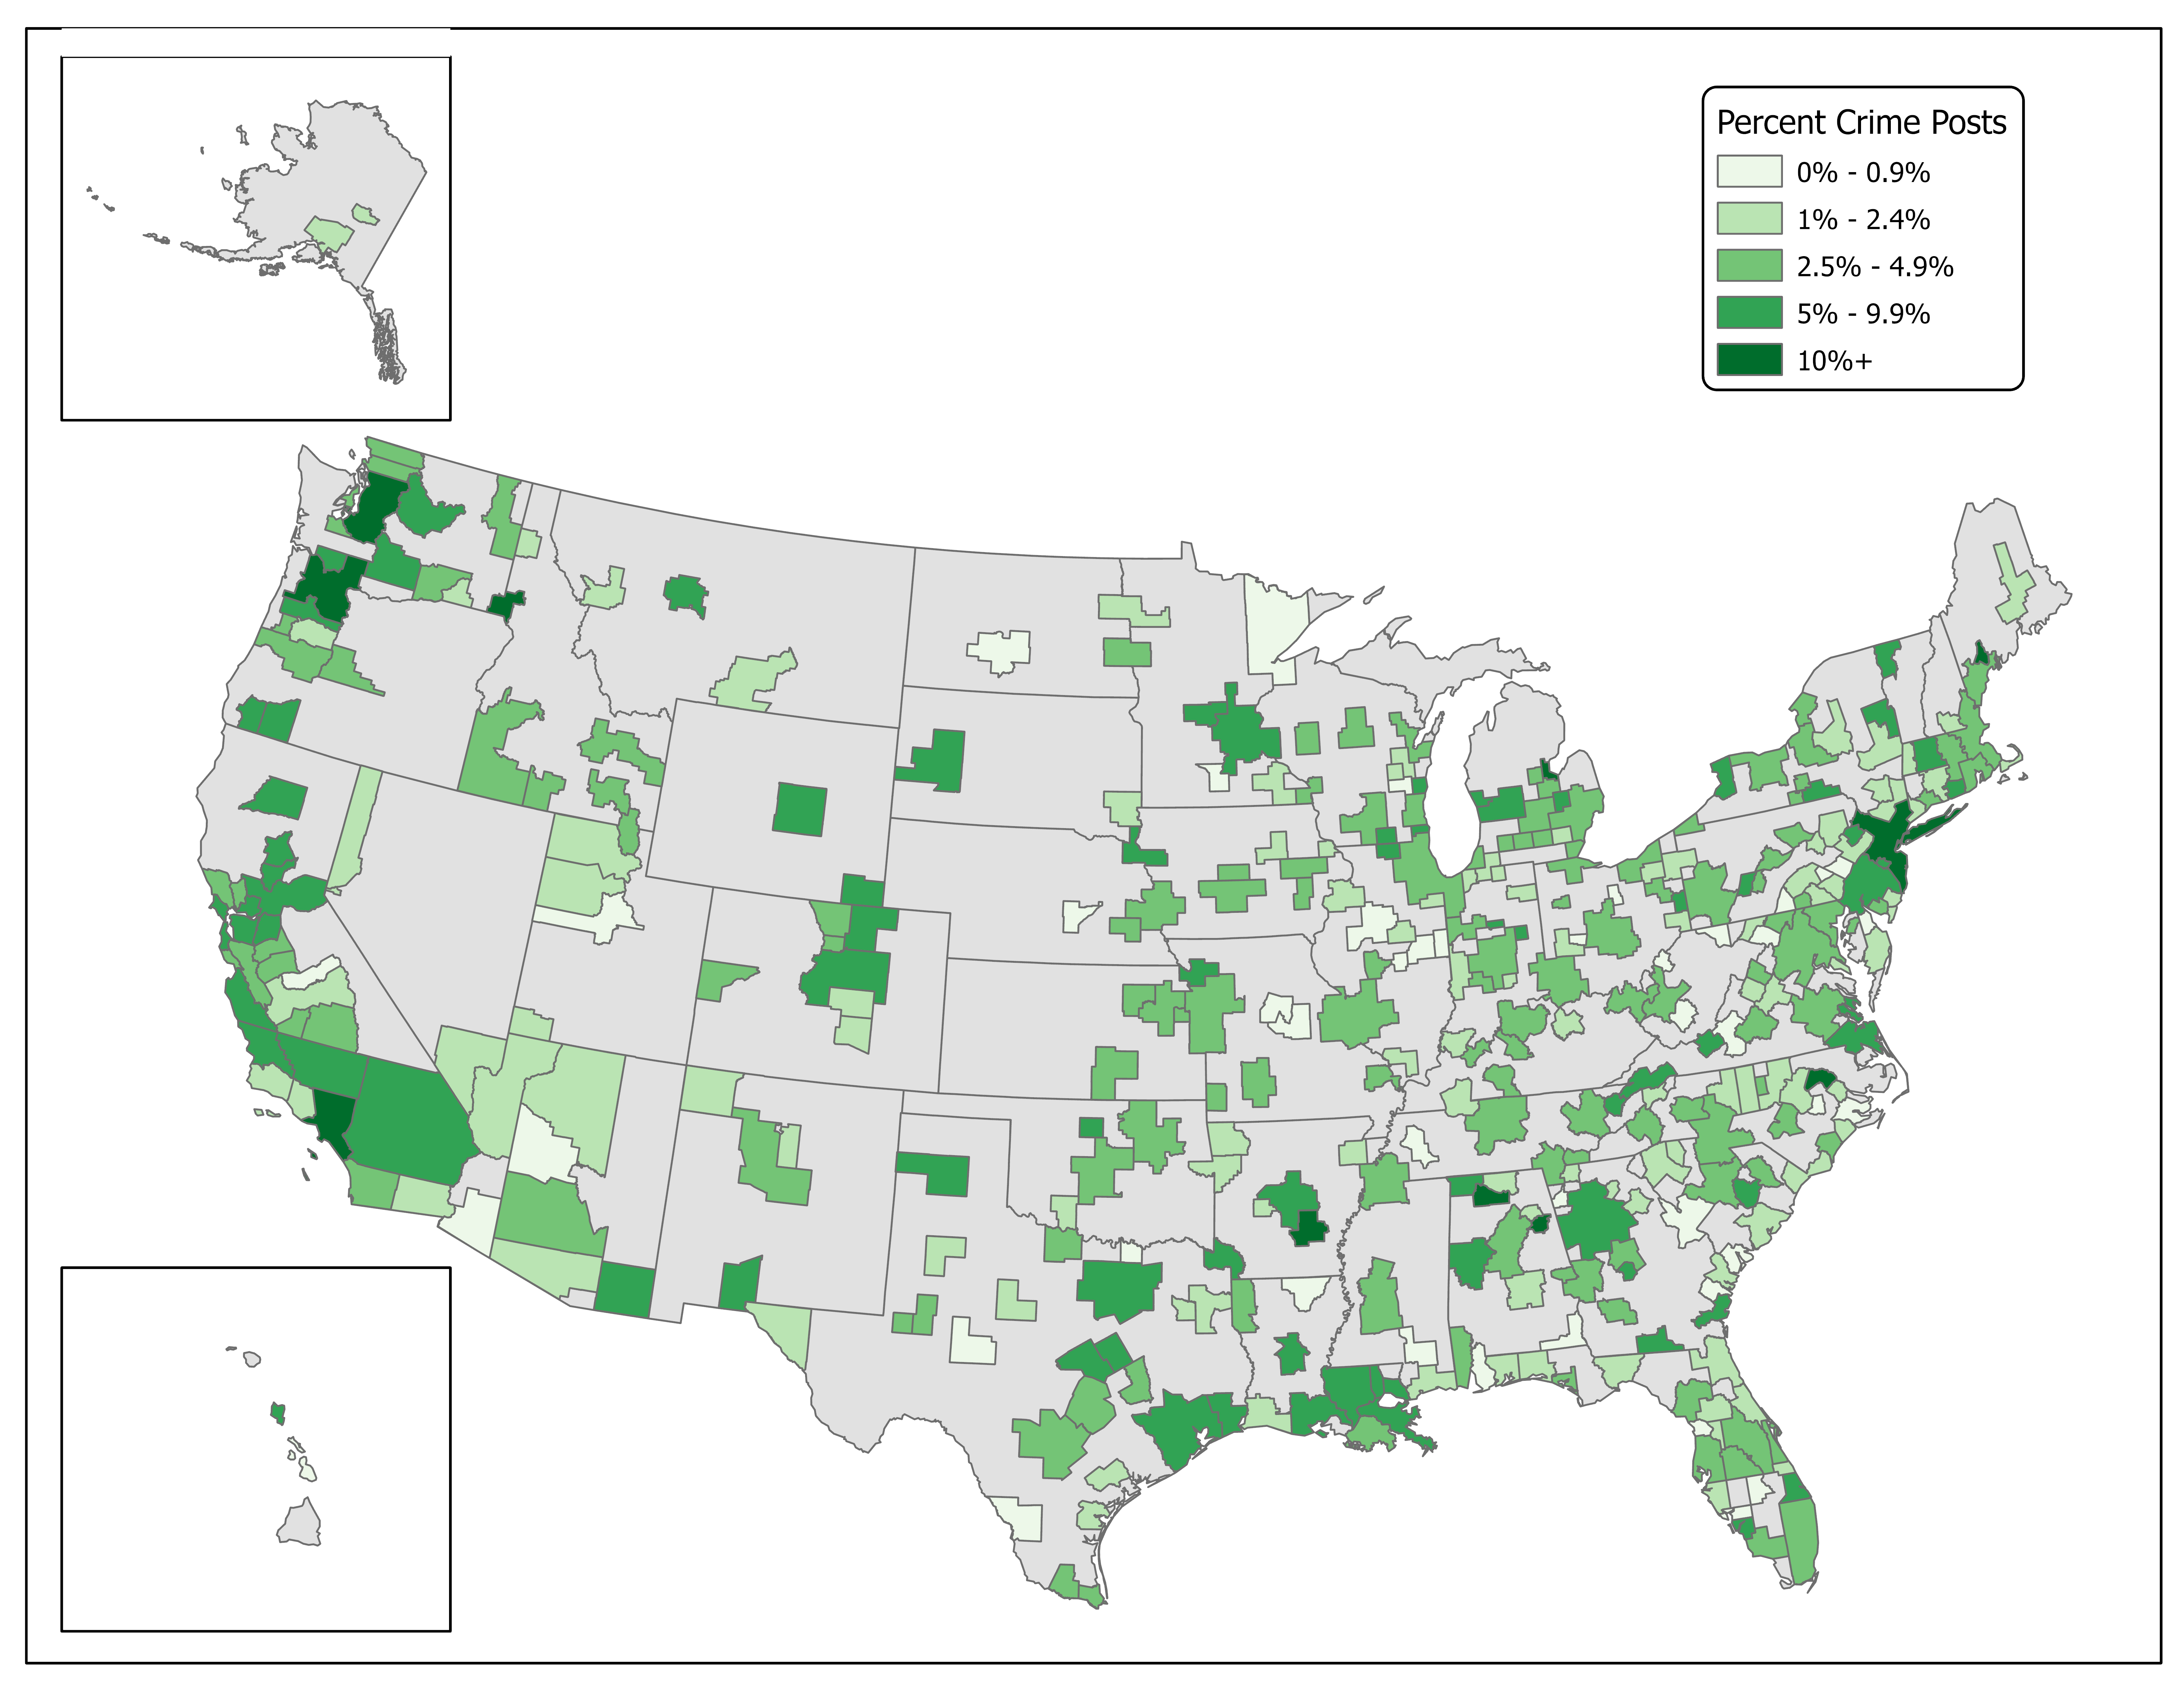
\includegraphics[width=\textwidth]{Images/PCrime.png}
    \caption{Map of crime discussion by MSA}
    \label{fig:map-1}
\end{figure}

\subsection{Crime Discussion and Population}

\par The 384 MSAs of the United States vary greatly in terms of their actual population sizes. Once the Urban Area that makes the core of the Statistical Area reaches a population of at least 50,000, a Metropolitan Area forms in the county (or counties) that the Urban Area lies in. As a result of this definition, we break down MSAs into the four categories based on size discussed previously: very small, small, medium, and large. We use these categorizations to help explain trends in data relating to MSA population sizes.

\par To identify any potential trends in the population data, we take the mean crime discussion value of each bucket category. Figure \ref{fig:graph-1} displays the average min-max normalization score for the percentage of crime discussion based on population size. Here, the very small population bucket contains 161 members with an average normalized score of 0.196, the small bucket contains 113 members with an average score of 0.173, the medium bucket contains 54 members with an average score of 0.166, and the large bucket contains 56 members with an average score of 0.260.

\begin{figure}[ht]
    \centering
    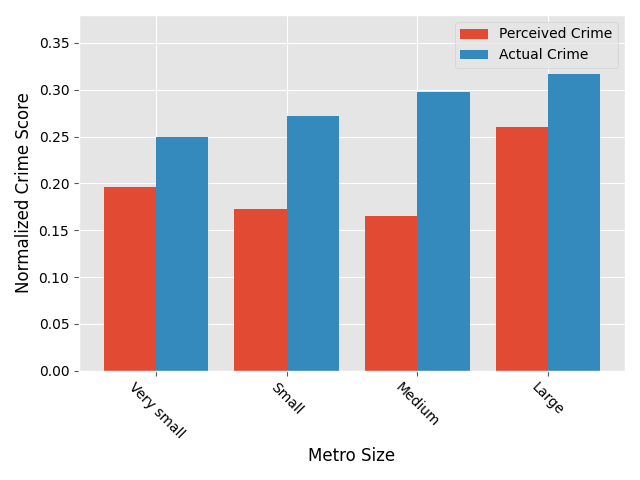
\includegraphics[width=0.75\textwidth]{Images/bar-population.png}
    \caption{Comparison of discussed crime and documented crime by population}
    \label{fig:graph-1}
\end{figure}

\par Figure \ref{fig:graph-1} provides average normalized scores for documented crime to compare trends to crime discussion. We can see that as population increases, documented crime rates gradually increase. This trend is semi-reflected in the crime discussion data. Crime discussion scores are roughly equivalent for the very small, small, and medium buckets. However, the large population bucket has a significantly higher crime discussion score than the other buckets. The large population bucket has a 6\% greater score than the medium population bucket when comparing documented crime data, but the large population bucket has a 56\% greater score than the medium population bucket when comparing crime discussion data.

\par Figure (REF) shows a cumulative distribution function of the data by population bucket. Here, we can see that the mean large population MSA has a fairly tight distribution, while the mean very small population MSA has a more spread out distribution.

(FIG)

\subsection{Crime Discussion and Politics}

\par Similarly to population data, political affiliation is one possible variable that can sway crime discussion. To measure this, we look at the results of the 2020 presidential election. We consider the number of votes that the Democratic and Republic parties received as stand-ins for liberal and conservative political views, respectfully. Political affiliation of the 384 MSAs is broken down into the five categories discussed earlier: very conservative, conservative, moderate, liberal, and very liberal. Figure \ref{fig:map-2} shows a map of the political affiliation of all Metropolitan Areas in the United States.

\begin{figure}[ht]
    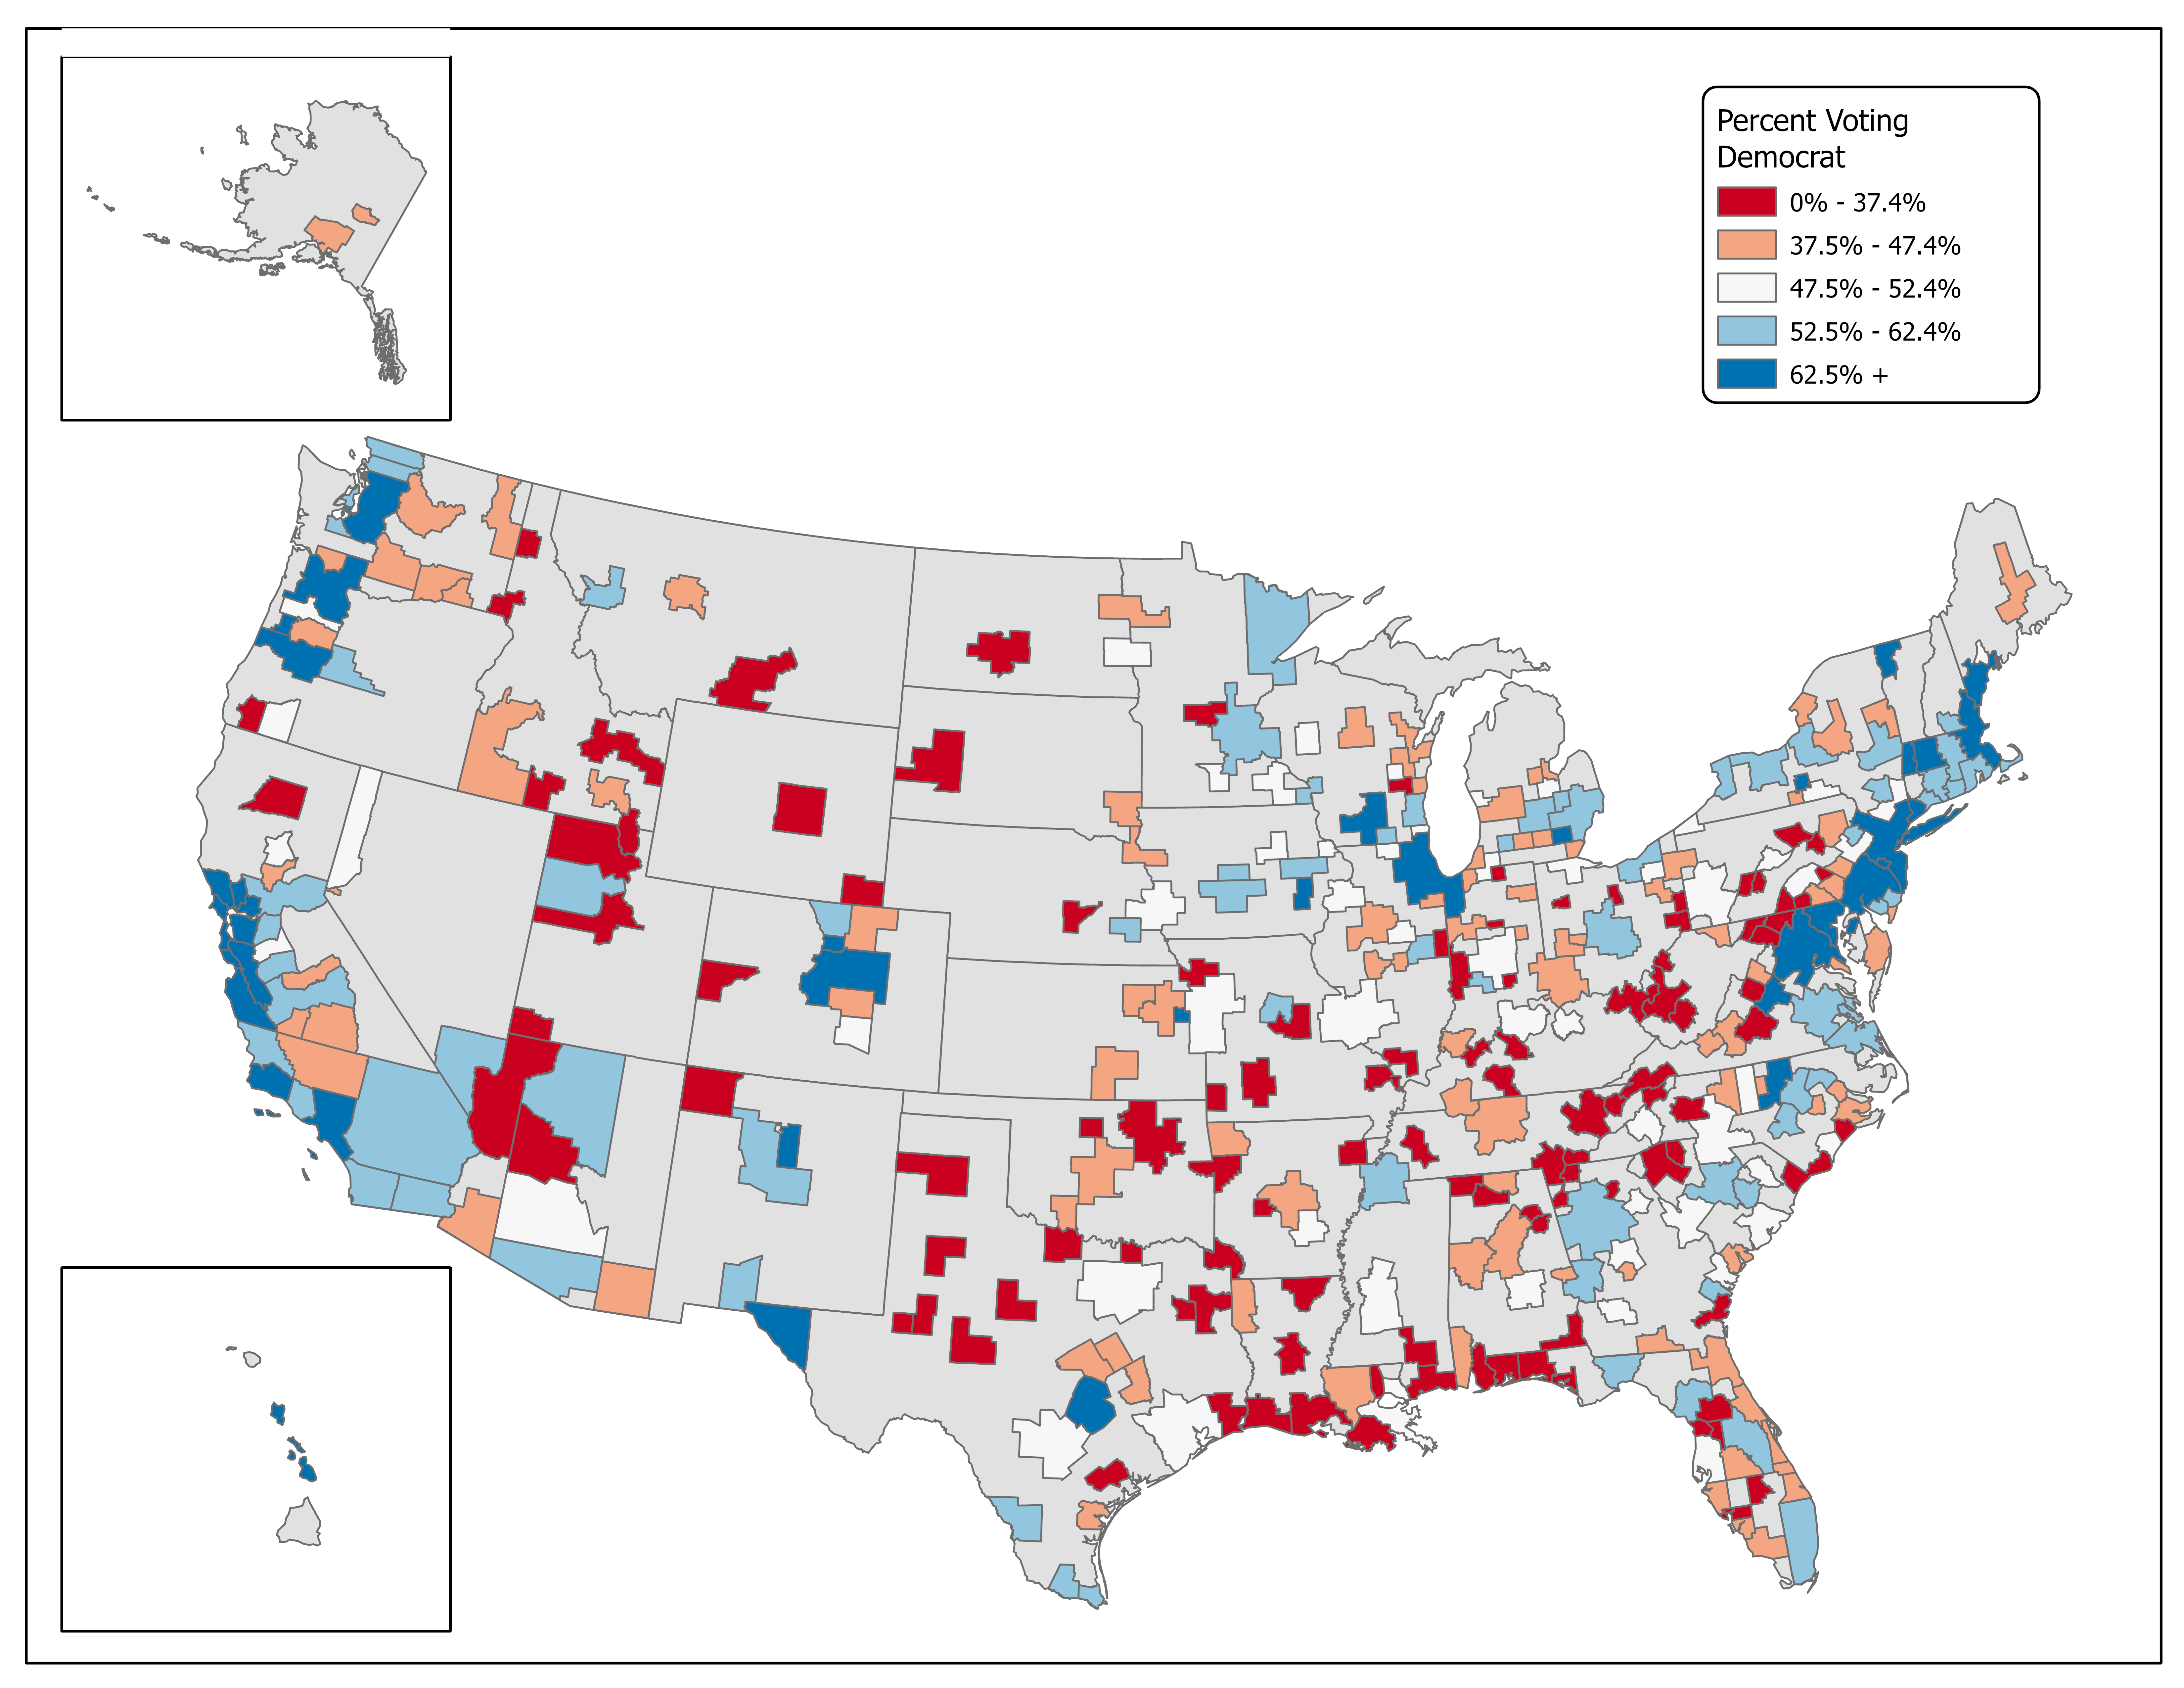
\includegraphics[width=\textwidth]{Images/pol.png}
    \caption{Map of 2020 Presidential Election Results by MSA}
    \label{fig:map-2}
\end{figure}

\par In identifying trends based on politics, we follow a familiar method and take the mean crime discussion value of each political class. Figure \ref{fig:graph-2} displays the average min-max normalization score for crime discussion and reported crime for each political class. Here, the very conservative bucket contains 112 members with a mean score of 0.170, the conservative bucket contains 103 members with a mean score of 0.179, the moderate bucket contains 57 members with a mean score of 0.207, the liberal bucket contains 73 members with a mean score of 0.201, and the very liberal bucket contains 39 members with a mean score of 0.274.

\begin{figure}[ht]
    \centering
    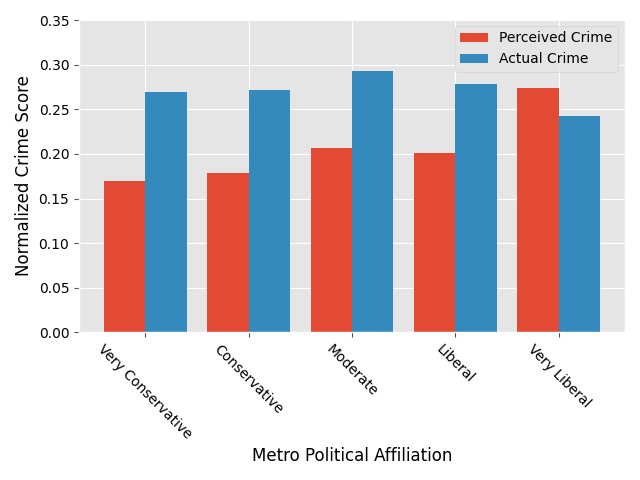
\includegraphics[width=0.75\textwidth]{Images/bar-politics.png}
    \caption{Comparison of discussed crime and documented crime by politics}
    \label{fig:graph-2}
\end{figure}

\par When looking at crime discussion rates, we can see that more liberal cities have the highest rates of crime discussion. The very liberal class has a 32\% higher crime discussion score than the next largest value. The two conservative political classes have the lowest crime discussion scores. However, these trends are not reflected in the documented crime rate scores. Figure \ref{fig:graph-2} shows that very liberal MSAs have a lower mean documented crime rate than more conservative areas. Very liberal areas are also the only class in which the crime discussion score is higher than the reported crime rate score.

\begin{figure}[!tbp]
  \centering
  \begin{minipage}[b]{0.45\textwidth}
    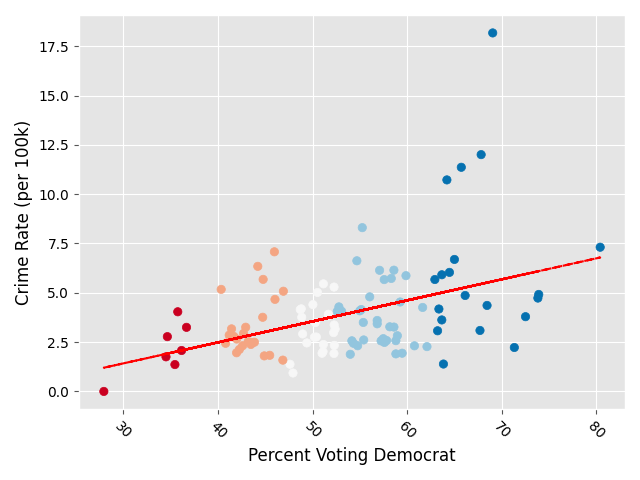
\includegraphics[width=\textwidth]{Images/scatter-politics-mid-large.png}
    \caption{Perceived crime by political leaning}
  \end{minipage}
  \hfill
  \begin{minipage}[b]{0.45\textwidth}
    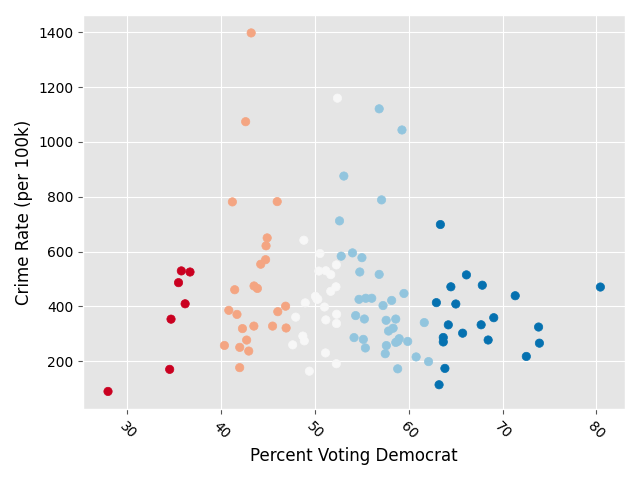
\includegraphics[width=\textwidth]{Images/scatter-crime-mid-large.png}
    \caption{Documented crime by political leaning}
  \end{minipage}
\end{figure}

\par Figure (REF) shows two scatterplots: one which shows the percent crime discussion in relation to politics among medium and large sized MSAs and the other which shows the documented crime rate among the same sample group in relation to politics. The shades of the dots represent their political class. From the trendline in the data, we can see that as areas become more liberal, their crime discussion percentages increase fairly rapidly. The most conservative member of the plot, Provo-Orem, UT, did not include a single post discussing crime, while more liberal areas such as Seattle, Los Angeles, Portland, and New York City had values over 10\%. In contrast, when looking at the documented violent crime rate among large and mid-size MSAs, more liberal areas generally have lower average crime rates. MSAs that lean conservative, such as Birmingham-Hoover, AL and Kansas City, MO-KS have among the highest crime rates, as well as more politically moderate cities, such as Memphis, TN-MS-AR.

\subsection{Crime Discussion and Reported Crime}

\chapter{User-level Analysis}
\par TODO

\section{Data Overview}
\par TODO: talk about sample of users and their data

\section{Methods}
\par TODO: talk about code design

\section{Results}
\par TODO: discuss results

\chapter{Conclusion}

\newpage
\chapter*{Appendix A}
\addcontentsline{toc}{chapter}{Appendix A}

% Appendix A - Metro, subreddit, population, hits
% Appendix B - Metro, population, pop class, Pcrime rate
% Appendix C - Metro, percent dem, pol class, pcrime rate
% Appendix D - Metro, normalized cr, normalized pcr
% Appendix E - Keywords

\newpage
\chapter*{Notes}
\addcontentsline{toc}{chapter}{Notes}

\newpage
\addcontentsline{toc}{chapter}{Bibliography/ References/ Works Cited}
\chapter*{Bibliography/ References/ Works Cited}
\setstretch{1.0}
\fontsize{10}{10pt} \selectfont
References should be single-spaced. The style and format for references should follow the style guide used for the rest of the dissertation. \newline \newline
Put an extra space in between entries.

% Remove lines 284, 287-288 and uncomment lines 291-292 while using template
%\renewcommand{\bibname}{Bibliography/References/Works Cited}
%\printbibliography

\end{document}
